\section{Our Proposed Tool}
In this section, we present our proposed tool, which consists of a
pair of algorithms, \ReReMi\ and \Siren. First, we explain how it
implement interactivity and visualization for redescription mining.
Then, we give a concrete illustration of its usage by means of a use
case. Throughout this section, we outline how the tool achieves goals
stated in the previous section by highlighting \emph{key
  features}. However, we are only able to achieve part of the goals---the rest are \emph{ch\^{a}teaux en Espagne}.

\subsection{The Algorithms}
\label{sec:algorithms}
\note{All explanations about the workings of ReReMi \& Siren here}

\Siren\ is
an interactive tool for mining and visualizing geospatial
redescriptions.\!\footnote{More details about \Siren's features, additional
  screenshots and a demonstration video are available online at
  \url{http://www.cs.helsinki.fi/u/galbrun/redescriptors/siren/}.}  At its core is the \ReReMi\ redescription mining
algorithm~\cite{galbrun11black,galbrun12black}.

This greedy algorithm
uses an efficient on-the-fly discretization technique to extend
redescription mining to categorical and numerical variables.
It considers queries over such variables that can be parsed in linear
order, without trees, with every variable allowed to appear only once.
They constitute a subset of Boolean formulae that
provides a good compromise between expressive power, difficulty of the
search, and interpretability.

Yet, the search space remains exponential and we still resort to
heuristic pruning.  We use a strategy similar to
beam-search to explore the solution space.  The basic idea is to
construct queries bottom-up, starting from singleton redescriptions
(i.e.\ both queries contain only one literal) and progressively
extending them by appending operators and
literals. % For example, we could start with a pair $(a,
% \lnot b)$, and try to extend it to $(a\land c, \lnot b)$, $(a \lor c,
% \lnot b)$, $(a \land \lnot c, \lnot b)$, etc.
After evaluating all possible one-step extensions, we select the best
candidates and extend them in turn. This process stops when no new
redescription can be generated.

Redescriptions with too high \pValue{} can be filtered out during the search.
We exploit some simple observations to make the computation of
accuracy more efficient. This allows to evaluate candidates faster,
which is particularly important for an interactive tool.  

Owing to his beam-search-like behaviour, \ReReMi{} is an
\emph{any-time} algorithm.  The intermediate redescriptions explored
during the search are returned at each step.  This way, the user is
able to see the candidates present in the beam and might stop the
extension process if he so wishes. He could possibly also remove a
candidate from the beam, cutting off a less promising branch from the
search.

In \Siren, threading is employed to delegate mining tasks to \ReReMi\
in the background. This preserves the tool's \emph{responsiveness}
while the communication is maintained to \emph{provide feedback} about
the ongoing mining, \emph{return results as they are obtained} and to
allow the user to directly interact with the process.  

Finally, \Siren\ allows automatic filtering of redundant
redescriptions. That is, redescriptions that cover approximately the
same area even if they have (somewhat) different sets of variables.
The user can select a redescription and ask \Siren\ either to filter
out all redescriptions that are redundant with respect to the selected
one, or to go through the whole list of redescriptions filtering out
all redescriptions that are redundant with respect to some
earlier-encountered (i.e.\ better) redescription. Naturally, the
decisions made by \Siren\ can be reverted whenever the user wishes to.

\note{This had been commented out... We need to say these things don't we?}
\Siren\ and \ReReMi\ are implemented in Python.  The interface is
built with the \texttt{wxPython} Open Source GUI toolkit, ensuring
cross-platform compatibility. 
 The \texttt{matplotlib} library enables
to generate high quality figures, seamlessly integrated in the
interface.  \Siren\ allows for simple editing of the redescriptions
thanks to flexible parsing of different representations. It can handle
any data provided in a compatible format.  

\subsection{Use Case}
\label{sec:scenarios}

\note{The old use-case scenario text is a good basis for this, but
  needs to be re-worked a lot.\\
Do we want to talk only about the functionalities that are already implemented, can be reasonably implemented in a short delay, or any wishable functionality? And insert links to the goal section... 
}

\note{Implemented and reasonably implementable, I'd say, plus possibly
  some discussion on wishful thinking (and why we might not be able to
meet some goals, too). Links back are very important, the whole
point. So this use-case must really highlight all the existing goals
we meet....}

We exemplify the usage of \Siren\ by going through a generic work-flow
of mining geospatial redescriptions, detailing typical steps in the
process.  This specific example concerns the application of \Siren\ on
the task of bioclimatic niche finding using data that describes
spatial areas of Europe, squares of side roughly 50 kilometers.  The
left hand side data contains information about the mammals that live
in these areas, while the right hand side consists of bioclimatic
variables\footnote{The data comes from two publicly available
  datasets: European mammal atlas~\cite{mitchell-jones99atlas} and
  Worldclim climate data~\cite{hijmans05very}.}.  Nonetheless, \Siren\
is a flexible tool that can be used with different datasets from
various application domains.

% A screenshot of the system,
% displaying a list of redescriptions with one
% particular redescription plotted on a map is shown in
% Figure~\ref{fig:both_panels}.

\prg{Initial redescription mining} A natural starting point for the
analysis of any given data is to use a redescription mining algorithm
to find an initial set of redescriptions.  This can be done within 
\Siren{} by running the extension mechanism on an empty redescription.
Following the principle of first providing an overview of the results
then focusing on specific items, the redescriptions found are
presented as a list from which the user can select a redescription of
his choice and to examine more closely and plot on the map.
Figure~\ref{fig:both_panels} shows two panels, containing an overview of
the current results as a list, in the background, and a single
redescription plotted on a map, in the foreground.
The list supports \emph{sorting} and \emph{filtering} on various criteria.

\prg{Extending a redescription} Sometimes the user wants to focus only
on one of the queries, on some particular variable of interest or on a
part of an existing redescription.  \Siren\ allows the user to
automatically extend a given redescription, i.e.\ let the algorithm
add new literals to the queries to make the redescription as accurate
as possible.
% (see Fig.~\ref{fig:extending}). 

In the climatic niche-finding task, for instance, we might select a
species, say, the Southwestern Water Vole and look for best extensions
starting from that single variable. Here, the best found extension has
accuracy $0.665$ (per Jaccard coefficient):
\begin{equation*}
%\footnotesize
\begin{array}{l}
\text{Southwestern Water Vole }\lor\text{ Gray Dwarf Hamster }\lor\text{ Savi's Pine Vole }\\[1mm]
\quad\lor\text{ Mediterranean Monk Seal}\\[3mm]
[11.2 \leq t_{3}^{+}] \land  [0.51 \leq t_{1}^{=} \leq 11.333]\land  [42.75 \leq p_{10}^{=} \leq 131.81] \\[1mm]
\quad\land [50.556 \leq p_{11}^{=} \leq 176.75],
\end{array}
\end{equation*}

This redescription indicates that areas where any of the four species
lives correspond to areas where the maximum temperature in March is
above $11.2$ degrees Celsius, the average temperature in January
between $0.51$ and $11.333$ degrees Celsius and the average
precipitations in October and November range from $42.75$ to $131.81$
millimeters and from $50.556$ to $176.75$ millimeters, respectively.

Returned extensions can be plotted on maps opened inside several
windows, so as to be \emph{visualized} side by side and compared as shown in
Figure~\ref{fig:comparison}.

\begin{figure}
  \centering
%%FIG%%
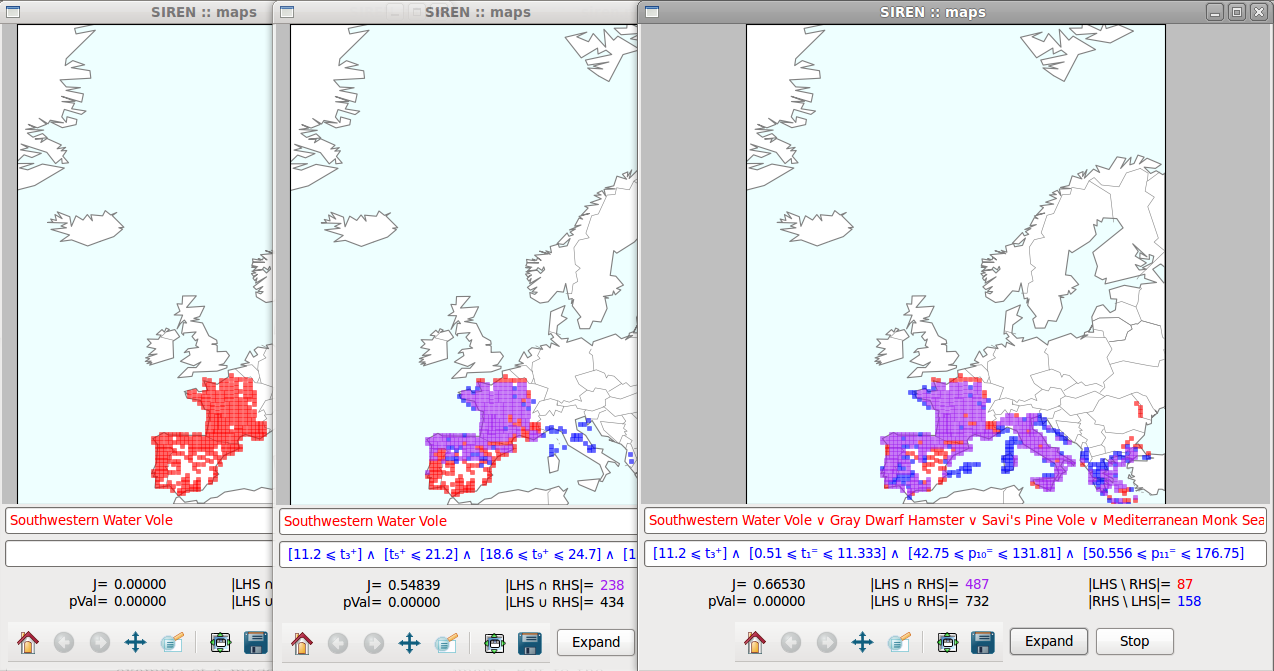
\includegraphics[width=0.7\textwidth]{screenshots/comparison}
  \caption{Several map panels. Comparing intermediate extensions automatically generated for a chosen starting variable. Red, blue and purple represents areas where only the left hand side query holds, only the right hand side query holds and where both queries hold, respectively.}
  \label{fig:comparison}
\end{figure}


\prg{Editing a redescription} It is typical that the user wants to
edit some of the obtained redescriptions. For example, some results
might be overly complex, or have exceedingly precise boundaries for
numerical variables. The user can easily select a redescription to
modify, open it in a map panel and edit it. Boundaries can be altered,
literals added or removed. \Siren\ \emph{instantly updates} the map and important
statistics (accuracy, $p$-value, etc.) of the redescription, allowing
the user to see the effects of the modifications immediately and
verify, e.g.\ whether the new redescription would still be acceptably
accurate.

Continuing with our example above, we might want to reduce the
precision of the climatic constraints to integers. We could edit the
query as follows:
\begin{equation*}
%\footnotesize
\begin{array}{l}
[11 \leq t_{3}^{+}] \land  [0 \leq t_{1}^{=} \leq 12]%\\[1mm]
%\quad
\land  [42 \leq p_{10}^{=} \leq 132] \land [50 \leq p_{11}^{=} \leq 177],
\end{array}
\end{equation*}
and obtain a redescription of slightly decreased accuracy. % of $0.659$.

\prg{Using subsets of variables} 
\Siren\ allows the user to specify variables to temporarily 
avoid when extending or mining redescriptions.
In our running example, we might want to force the
algorithm to search alternative redescriptions that do not involve any
 precipitation. For that purpose, we simply unselect all such
variables before running the extension anew. We will obtain the best
extensions containing only temperatures in the bioclimatic query, such
as the following redescription of accuracy $0.653$:
\begin{equation*}
%\footnotesize
\begin{array}{l}
\text{Southwestern Water Vole }\lor\text{ Cape Hare }\lor\text{ Savi's Pine Vole }\\[1mm]
\quad\lor\text{ Mediterranean Monk Seal}\\[3mm]
( [11.2 \leq t_{3}^{+}] \land  [20.1 \leq t_{7}^{+} \leq 32.9] %\\[1mm] 
%\quad 
\land  [0.51 \leq t_{1}^{=} \leq 11.333]) \lor  [34.0 \leq t_{8}^{+}].
\end{array}
\end{equation*}

Note that this redescription was not returned previously since the
beam search focused on better ones involving precipitation variables.
This feature allows the user to specify additional constraints,
thereby \emph{tuning the mining process} according to his interest and
what appears most promising during the analysis.

\prg{Filtering redundant redescriptions}
\label{sec:filt-redund-redescr}
The results returned during the extension
mentioned previously may contain many redundant redescriptions found
at different steps. We can easily sort them, e.g.\ by accuracy, select
one of interest and filter all the following results redundant with respect to it.

\prg{Sharing the results}
\label{sec:sharing-results}
Finally, \Siren\ facilitates \emph{distributing} the results:
redescriptions can be exported in easy-to-read format and the
maps associated to redescriptions can be readily converted to
publication-ready graphics. 

%%% Local Variables: 
%%% mode: latex
%%% TeX-master: "siren_iid"
%%% End: 

% LocalWords:  iid
